\subsubsection{levelplot()}
Levelplot is the \texttt{lattice} answer to plotting surfaces. If you really want to understand the guts of what is going on this code, then you should really read the Jakoby material linked earlier in this document. I personally do not use \texttt{lattice} often, precicely because the specification of axes, labels and overplotting is a chore. Here I first display the default output so that you're not shocked when you first try it. On the positive side, note that the aspect ratio by default maintains a 45 degree angle over x and y values, plus there is a color strip legend by default. This we like. The default color ramp is not so useful, nor are the crowded tick labels.



\begin{Houtput}
\hspace*{\fill}\\
\hlstd{}\ttfamily\noindent
\hlprompt{\usebox{\hlnormalsizeboxgreaterthan}{\ }}\hlfunctioncall{library}\hlkeyword{(}\hlsymbol{lattice}\hlkeyword{)}\mbox{}
\normalfont
\hspace*{\fill}\\
\hlstd{}\ttfamily\noindent
\hlprompt{\usebox{\hlnormalsizeboxgreaterthan}{\ }}\hlfunctioncall{levelplot}\hlkeyword{(}\hlfunctioncall{log}\hlkeyword{(}\hlsymbol{MxMat}\hlkeyword{)}\hlkeyword{,}\hlargument{main}\hlargument{=}\hlstring{"Default{\ }levelplot()"}\hlkeyword{)}\mbox{}
\normalfont
\hspace*{\fill}\\
\hlstd{}
\end{Houtput}



\begin{figure}
\centering
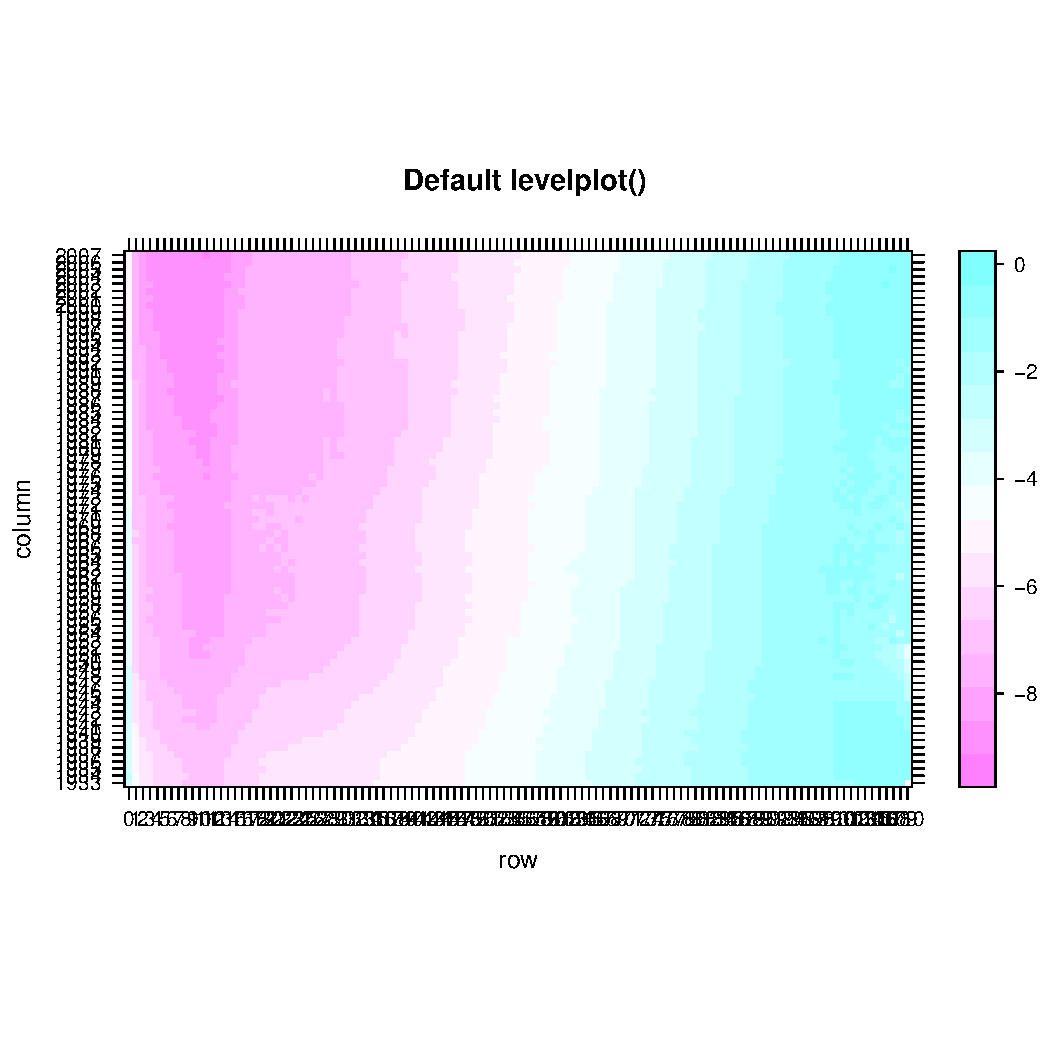
\includegraphics[width=4.5in,height=4.5in]{figs/latticedefault.pdf}
\caption{\texttt{levelplot()} function, leaving all defaults.}
\end{figure}

% hidden stuff that gets used


The steps in this code are in need of some explanation, I admit. First, you need to know that lattice does not (easily) let you modify a plot once it's made, so you need to (or it's best to) specify everything from within a single function call. For this reason, all of the Lexis reference line overplotting needs to get pre-written into a custom function, \texttt{lexisreferencelines()}, called a \textit{panel} function that later gets called within the main lattice function, in this case \texttt{levelplot()}. To understand this more, please refer to the online material mentioned before. The other quirks I'll explain here. First, \texttt{levelplot()} will take a variety of things as its main data argument, not necessarily a matrix\footnote{This could also be done with a formula and \texttt{data.frame} in long format, which is not shown here.}. Here we gave it a matrix (the transpose of \texttt{log(MxMat)}), just as with \texttt{image()}, but we need requires a few extra steps in order to get the axes right.\\

When specifying a matrix, by default \texttt{levelplot()} will consider your x and y values to start at 0 and count upward, which is \textit{almost} correct for ages and very far off for years. This we rectify by supplying the \texttt{row.values} and \texttt{column.values} arguments. Like other surface functions in R, each cell will be centered on its assigned x and y value, and so in order to render properly, we shift the x and y values by .5, but specify the x and y limits to stretch over the entire data range (1993-2008 (end of 2007), and 0-111 (110+)). This is a very fine point, easy to not notice, but essential to get right if you want the image to be exact. Next we specify the color ramp with \texttt{color.regions}, just as we did \texttt{col} in the other functions. Color strip legend arguments get sent as a list to the \texttt{colorkey} argument: notice that I give the same values, and they are all correctly plotted (better than \texttt{image.plot()} already). The \texttt{scales} argument is the way to be precise about axis labelling in \texttt{lattice}: it is also give as a list, with elements x and y. If omitted, the plot renders just fine, but you only get axis labels every 20 ages/years\footnote{Actually we also got rather rough labels with \texttt{axis()} before, but this could have been fixed by manually labelling with \texttt{text()}.}. Finally, and most importantly, we specify a panel function, in this case our \texttt{lexisreferencelines} function. Panel functions tend to follow this form, and can be very complex if desired.

\begin{Houtput}
\hspace*{\fill}\\
\hlstd{}\ttfamily\noindent
\hlprompt{\usebox{\hlnormalsizeboxgreaterthan}{\ }}\hlfunctioncall{library}\hlkeyword{(}\hlsymbol{lattice}\hlkeyword{)}\mbox{}
\normalfont
\hspace*{\fill}\\
\hlstd{}\ttfamily\noindent
\hlprompt{\usebox{\hlnormalsizeboxgreaterthan}{\ }}\hlsymbol{brks}{\ }\hlassignement{\usebox{\hlnormalsizeboxlessthan}-}{\ }\hlfunctioncall{approx}\hlkeyword{(}\hlfunctioncall{log}\hlkeyword{(}\hlfunctioncall{c}\hlkeyword{(}\hlnumber{1e-5}\hlkeyword{,}\hlnumber{1}\hlkeyword{)}\hlkeyword{)}\hlkeyword{,}\hlargument{n}\hlargument{=}\hlnumber{21}\hlkeyword{)}\hlkeyword{\usebox{\hlnormalsizeboxdollar}}\hlsymbol{y}\mbox{}
\normalfont
\hspace*{\fill}\\
\hlstd{}\ttfamily\noindent
\hlprompt{\usebox{\hlnormalsizeboxgreaterthan}{\ }}\hlsymbol{legendlabs}{\ }\hlassignement{\usebox{\hlnormalsizeboxlessthan}-}{\ }\hlfunctioncall{c}\hlkeyword{(}\hlnumber{1}\hlkeyword{,}\hlnumber{.1}\hlkeyword{,}\hlnumber{.01}\hlkeyword{,}\hlnumber{1e-3}\hlkeyword{,}\hlnumber{1e-4}\hlkeyword{,}\hlnumber{1e-5}\hlkeyword{)}\mbox{}
\normalfont
\hspace*{\fill}\\
\hlstd{}\ttfamily\noindent
\hlprompt{\usebox{\hlnormalsizeboxgreaterthan}{\ }}\hlcomment{\usebox{\hlnormalsizeboxhash}{\ }panel{\ }function{\ }for{\ }inside{\ }levelplot():}\hspace*{\fill}\\
\hlstd{}\hlprompt{\usebox{\hlnormalsizeboxgreaterthan}{\ }}\hlsymbol{lexisreferencelines}{\ }\hlassignement{\usebox{\hlnormalsizeboxlessthan}-}{\ }\hlkeyword{function}\hlkeyword{(}\hlformalargs{...}\hlkeyword{)}{\ }\hlkeyword{\usebox{\hlnormalsizeboxopenbrace}}\hspace*{\fill}\\
\hlstd{}\hlprompt{{\ }}{\ }{\ }{\ }{\ }{\ }{\ }{\ }{\ }\hlfunctioncall{panel.levelplot}\hlkeyword{(}\hlsymbol{...}\hlkeyword{)}\hspace*{\fill}\\
\hlstd{}\hlprompt{{\ }}{\ }{\ }{\ }{\ }{\ }{\ }{\ }{\ }\hlcomment{\usebox{\hlnormalsizeboxhash}{\ }cohort{\ }lines{\ }(same{\ }cmat{\ }as{\ }before)}\hspace*{\fill}\\
\hlstd{}\hlprompt{{\ }}{\ }{\ }{\ }{\ }{\ }{\ }{\ }{\ }\hlfunctioncall{panel.segments}\hlkeyword{(}\hlsymbol{cmat}\hlkeyword{[}\hlnumber{1}\hlkeyword{,}\hlkeyword{]}\hlkeyword{,}\hlsymbol{cmat}\hlkeyword{[}\hlnumber{2}\hlkeyword{,}\hlkeyword{]}\hlkeyword{,}\hlsymbol{cmat}\hlkeyword{[}\hlnumber{3}\hlkeyword{,}\hlkeyword{]}\hlkeyword{,}\hlsymbol{cmat}\hlkeyword{[}\hlnumber{4}\hlkeyword{,}\hlkeyword{]}\hlkeyword{,}\hlargument{col}\hlargument{=}\hlstring{"\usebox{\hlnormalsizeboxhash}00000040"}\hlkeyword{)}\hspace*{\fill}\\
\hlstd{}\hlprompt{{\ }}{\ }{\ }{\ }{\ }{\ }{\ }{\ }{\ }\hlcomment{\usebox{\hlnormalsizeboxhash}{\ }period{\ }lines}\hspace*{\fill}\\
\hlstd{}\hlprompt{{\ }}{\ }{\ }{\ }{\ }{\ }{\ }{\ }{\ }\hlfunctioncall{panel.segments}\hlkeyword{(}\hlfunctioncall{seq}\hlkeyword{(}\hlnumber{1940}\hlkeyword{,}\hlnumber{2000}\hlkeyword{,}\hlargument{by}\hlargument{=}\hlnumber{10}\hlkeyword{)}\hlkeyword{,}\hlnumber{0}\hlkeyword{,}\hlfunctioncall{seq}\hlkeyword{(}\hlnumber{1940}\hlkeyword{,}\hlnumber{2000}\hlkeyword{,}\hlargument{by}\hlargument{=}\hlnumber{10}\hlkeyword{)}\hlkeyword{,}\hlnumber{111}\hlkeyword{,}\hlargument{col}\hlargument{=}\hlstring{"\usebox{\hlnormalsizeboxhash}00000040"}\hlkeyword{)}\hspace*{\fill}\\
\hlstd{}\hlprompt{{\ }}{\ }{\ }{\ }{\ }{\ }{\ }{\ }{\ }\hlcomment{\usebox{\hlnormalsizeboxhash}{\ }age{\ }lines}\hspace*{\fill}\\
\hlstd{}\hlprompt{{\ }}{\ }{\ }{\ }{\ }{\ }{\ }{\ }{\ }\hlfunctioncall{panel.segments}\hlkeyword{(}\hlnumber{1933}\hlkeyword{,}\hlfunctioncall{seq}\hlkeyword{(}\hlnumber{0}\hlkeyword{,}\hlnumber{111}\hlkeyword{,}\hlargument{by}\hlargument{=}\hlnumber{10}\hlkeyword{)}\hlkeyword{,}\hlnumber{2008}\hlkeyword{,}\hlfunctioncall{seq}\hlkeyword{(}\hlnumber{0}\hlkeyword{,}\hlnumber{111}\hlkeyword{,}\hlargument{by}\hlargument{=}\hlnumber{10}\hlkeyword{)}\hlkeyword{,}\hlargument{col}\hlargument{=}\hlstring{"\usebox{\hlnormalsizeboxhash}00000040"}\hlkeyword{)}\hspace*{\fill}\\
\hlstd{}\hlprompt{{\ }}\hlkeyword{\usebox{\hlnormalsizeboxclosebrace}}\mbox{}
\normalfont
\hspace*{\fill}\\
\hlstd{}\ttfamily\noindent
\hlprompt{\usebox{\hlnormalsizeboxgreaterthan}{\ }}\hlcomment{\usebox{\hlnormalsizeboxhash}{\ }the{\ }main{\ }surface{\ }function:}\hspace*{\fill}\\
\hlstd{}\hlprompt{\usebox{\hlnormalsizeboxgreaterthan}{\ }}\hlfunctioncall{print}\hlkeyword{(}\hspace*{\fill}\\
\hlstd{}\hlprompt{{\ }}\hlfunctioncall{levelplot}\hlkeyword{(}\hlfunctioncall{t}\hlkeyword{(}\hlfunctioncall{log}\hlkeyword{(}\hlsymbol{MxMat}\hlkeyword{)}\hlkeyword{)}\hlkeyword{,}\hspace*{\fill}\\
\hlstd{}\hlprompt{{\ }}{\ }{\ }{\ }{\ }{\ }{\ }{\ }{\ }\hlargument{row.values}\hlargument{=}\hlnumber{1933.5}\hlkeyword{:}\hlnumber{2007.5}\hlkeyword{,}\hspace*{\fill}\\
\hlstd{}\hlprompt{{\ }}{\ }{\ }{\ }{\ }{\ }{\ }{\ }{\ }\hlargument{column.values}\hlargument{=}\hlnumber{0.5}\hlkeyword{:}\hlnumber{110.5}\hlkeyword{,}\hspace*{\fill}\\
\hlstd{}\hlprompt{{\ }}{\ }{\ }{\ }{\ }{\ }{\ }{\ }{\ }\hlargument{xlim}\hlargument{=}\hlfunctioncall{c}\hlkeyword{(}\hlnumber{1933}\hlkeyword{,}\hlnumber{2008}\hlkeyword{)}\hlkeyword{,}\hspace*{\fill}\\
\hlstd{}\hlprompt{{\ }}{\ }{\ }{\ }{\ }{\ }{\ }{\ }{\ }\hlargument{ylim}\hlargument{=}\hlfunctioncall{c}\hlkeyword{(}\hlnumber{0}\hlkeyword{,}\hlnumber{111}\hlkeyword{)}\hlkeyword{,}\hspace*{\fill}\\
\hlstd{}\hlprompt{{\ }}{\ }{\ }{\ }{\ }{\ }{\ }{\ }{\ }\hlargument{at}\hlargument{=}\hlsymbol{brks}\hlkeyword{,}\hspace*{\fill}\\
\hlstd{}\hlprompt{{\ }}{\ }{\ }{\ }{\ }{\ }{\ }{\ }{\ }\hlargument{col.regions}\hlargument{=}\hlfunctioncall{rev}\hlkeyword{(}\hlfunctioncall{heat.colors}\hlkeyword{(}\hlnumber{20}\hlkeyword{)}\hlkeyword{)}\hlkeyword{,}\hspace*{\fill}\\
\hlstd{}\hlprompt{{\ }}{\ }{\ }{\ }{\ }{\ }{\ }{\ }{\ }\hlargument{colorkey}\hlargument{=}\hlfunctioncall{list}\hlkeyword{(}\hlargument{at}\hlargument{=}\hlsymbol{brks}\hlkeyword{,}\hspace*{\fill}\\
\hlstd{}\hlprompt{{\ }}{\ }{\ }{\ }{\ }{\ }{\ }{\ }{\ }{\ }{\ }{\ }{\ }{\ }{\ }{\ }{\ }{\ }{\ }{\ }{\ }{\ }{\ }{\ }{\ }\hlargument{labels}\hlargument{=}\hlfunctioncall{list}\hlkeyword{(}\hlargument{at}\hlargument{=}\hlfunctioncall{log}\hlkeyword{(}\hlsymbol{legendlabs}\hlkeyword{)}\hlkeyword{,}\hspace*{\fill}\\
\hlstd{}\hlprompt{{\ }}{\ }{\ }{\ }{\ }{\ }{\ }{\ }{\ }{\ }{\ }{\ }{\ }{\ }{\ }{\ }{\ }{\ }{\ }{\ }{\ }{\ }{\ }{\ }{\ }{\ }{\ }{\ }{\ }{\ }{\ }{\ }{\ }{\ }{\ }{\ }{\ }{\ }{\ }{\ }{\ }\hlargument{labels}\hlargument{=}\hlsymbol{legendlabs}\hlkeyword{)}\hspace*{\fill}\\
\hlstd{}\hlprompt{{\ }}{\ }{\ }{\ }{\ }{\ }{\ }{\ }{\ }\hlkeyword{)}\hlkeyword{,}\hspace*{\fill}\\
\hlstd{}\hlprompt{{\ }}{\ }{\ }{\ }{\ }{\ }{\ }{\ }{\ }\hlargument{scales}\hlargument{=}\hlfunctioncall{list}\hlkeyword{(}\hlargument{x}\hlargument{=}\hlfunctioncall{list}\hlkeyword{(}\hlargument{at}\hlargument{=}\hlfunctioncall{seq}\hlkeyword{(}\hlnumber{1940}\hlkeyword{,}\hlnumber{2000}\hlkeyword{,}\hlargument{by}\hlargument{=}\hlnumber{10}\hlkeyword{)}\hlkeyword{,}\hspace*{\fill}\\
\hlstd{}\hlprompt{{\ }}{\ }{\ }{\ }{\ }{\ }{\ }{\ }{\ }{\ }{\ }{\ }{\ }{\ }{\ }{\ }{\ }{\ }{\ }{\ }{\ }{\ }{\ }{\ }{\ }{\ }{\ }{\ }{\ }{\ }{\ }{\ }{\ }{\ }{\ }{\ }{\ }{\ }{\ }{\ }{\ }\hlargument{labels}\hlargument{=}\hlfunctioncall{seq}\hlkeyword{(}\hlnumber{1940}\hlkeyword{,}\hlnumber{2000}\hlkeyword{,}\hlargument{by}\hlargument{=}\hlnumber{10}\hlkeyword{)}\hlkeyword{)}\hlkeyword{,}\hspace*{\fill}\\
\hlstd{}\hlprompt{{\ }}{\ }{\ }{\ }{\ }{\ }{\ }{\ }{\ }{\ }{\ }{\ }{\ }{\ }{\ }{\ }{\ }{\ }{\ }{\ }{\ }{\ }{\ }{\ }{\ }\hlargument{y}\hlargument{=}\hlfunctioncall{list}\hlkeyword{(}\hlargument{at}\hlargument{=}\hlfunctioncall{seq}\hlkeyword{(}\hlnumber{0}\hlkeyword{,}\hlnumber{110}\hlkeyword{,}\hlargument{by}\hlargument{=}\hlnumber{10}\hlkeyword{)}\hlkeyword{)}\hlkeyword{,}\hspace*{\fill}\\
\hlstd{}\hlprompt{{\ }}{\ }{\ }{\ }{\ }{\ }{\ }{\ }{\ }{\ }{\ }{\ }{\ }{\ }{\ }{\ }{\ }{\ }{\ }{\ }{\ }{\ }{\ }{\ }{\ }\hlargument{labels}\hlargument{=}\hlfunctioncall{seq}\hlkeyword{(}\hlnumber{0}\hlkeyword{,}\hlnumber{110}\hlkeyword{,}\hlargument{by}\hlargument{=}\hlnumber{10}\hlkeyword{)}\hlkeyword{)}\hlkeyword{,}\hspace*{\fill}\\
\hlstd{}\hlprompt{{\ }}{\ }{\ }{\ }{\ }{\ }{\ }{\ }{\ }\hlargument{xlab}\hlargument{=}\hlstring{"Year"}\hlkeyword{,}\hspace*{\fill}\\
\hlstd{}\hlprompt{{\ }}{\ }{\ }{\ }{\ }{\ }{\ }{\ }{\ }\hlargument{ylab}\hlargument{=}\hlstring{"Age"}\hlkeyword{,}\hspace*{\fill}\\
\hlstd{}\hlprompt{{\ }}{\ }{\ }{\ }{\ }{\ }{\ }{\ }{\ }\hlargument{main}\hlargument{=}\hlstring{"Same{\ }surface{\ }plot{\ }using{\ }lattice{\ }levelplot()"}\hlkeyword{,}\hspace*{\fill}\\
\hlstd{}\hlprompt{{\ }}{\ }{\ }{\ }{\ }{\ }{\ }{\ }{\ }\hlargument{panel}\hlargument{=}\hlsymbol{lexisreferencelines}\hspace*{\fill}\\
\hlstd{}\hlprompt{{\ }}\hlkeyword{)}\hspace*{\fill}\\
\hlstd{}\hlprompt{{\ }}\hlkeyword{)}\mbox{}
\normalfont
\hspace*{\fill}\\
\hlstd{}
\end{Houtput}



\begin{figure}[H]
\centering
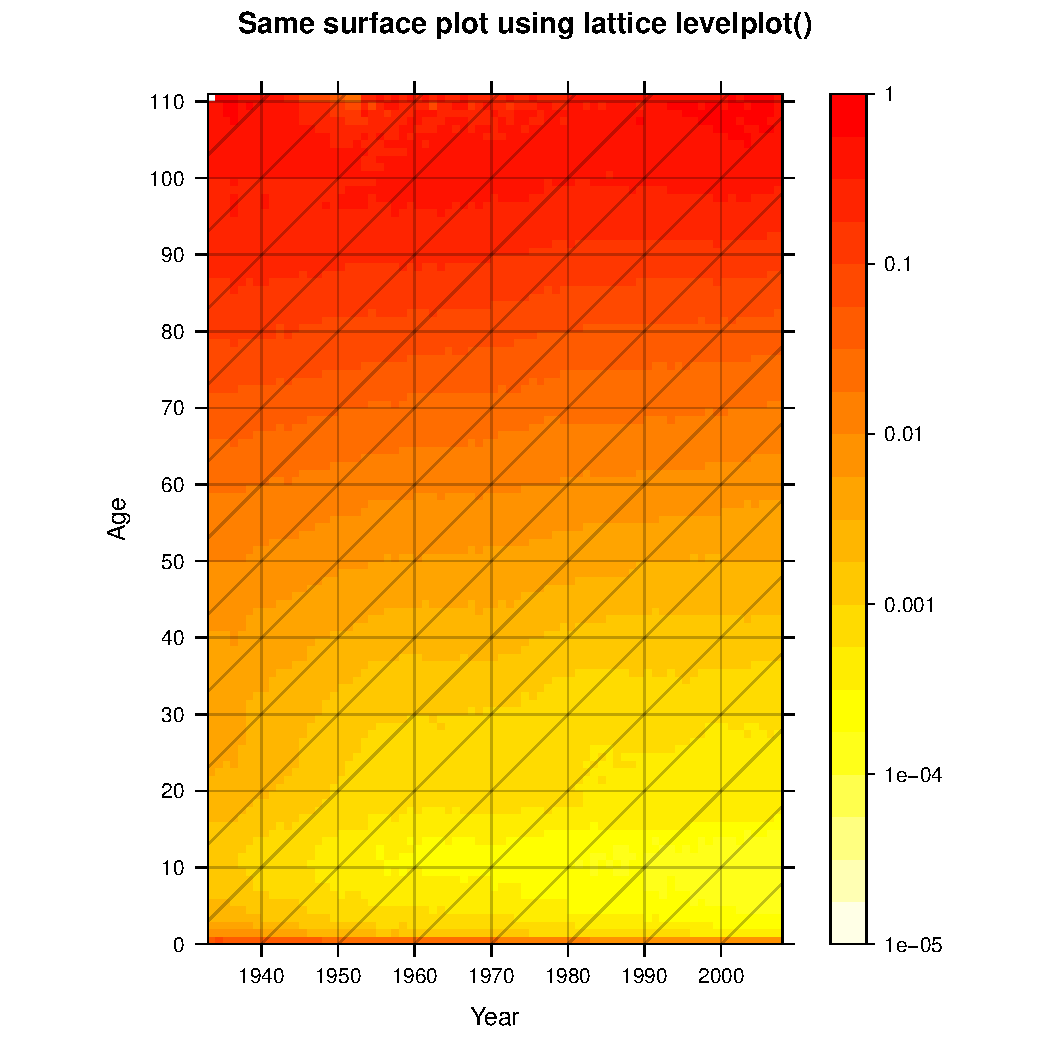
\includegraphics[width=4.5in,height=4.5in]{figs/latticegood.pdf}
\caption{\texttt{levelplot()} function, tweaked to produce a Lexis surface.}
\end{figure}

Sometimes you see surfaces displayed via contour plots that resemble topographic maps. These may or may not be desirable for your particular surface. The \texttt{contourplot()} function in lattice is a companion to \texttt{levelplot()}, and works in much the same way. A shortcut that I used to produce the below plot was to simply add the argument $\texttt{contour=TRUE}$ to the \texttt{levelplot()} list of arguments. Notice that the contour lines themselves are smooth interpolations and do not follow cell borders exactly. This can often help piont out details in the surface, most often period effects, that can go unnoticed on color-only surfaces. Local maxima and minima are also marked. In my opinion the following plot is locally more legible, but on the whole suffers from information overload, since the contour lines pick up noise from ages. You could clean up the image by not overlaying Lexis lines, but then its difficult for your eyes to keep track of age, period and cohort. Whether or not to use contour lines is thus a matter of judgement.





\begin{figure}[H]
\centering
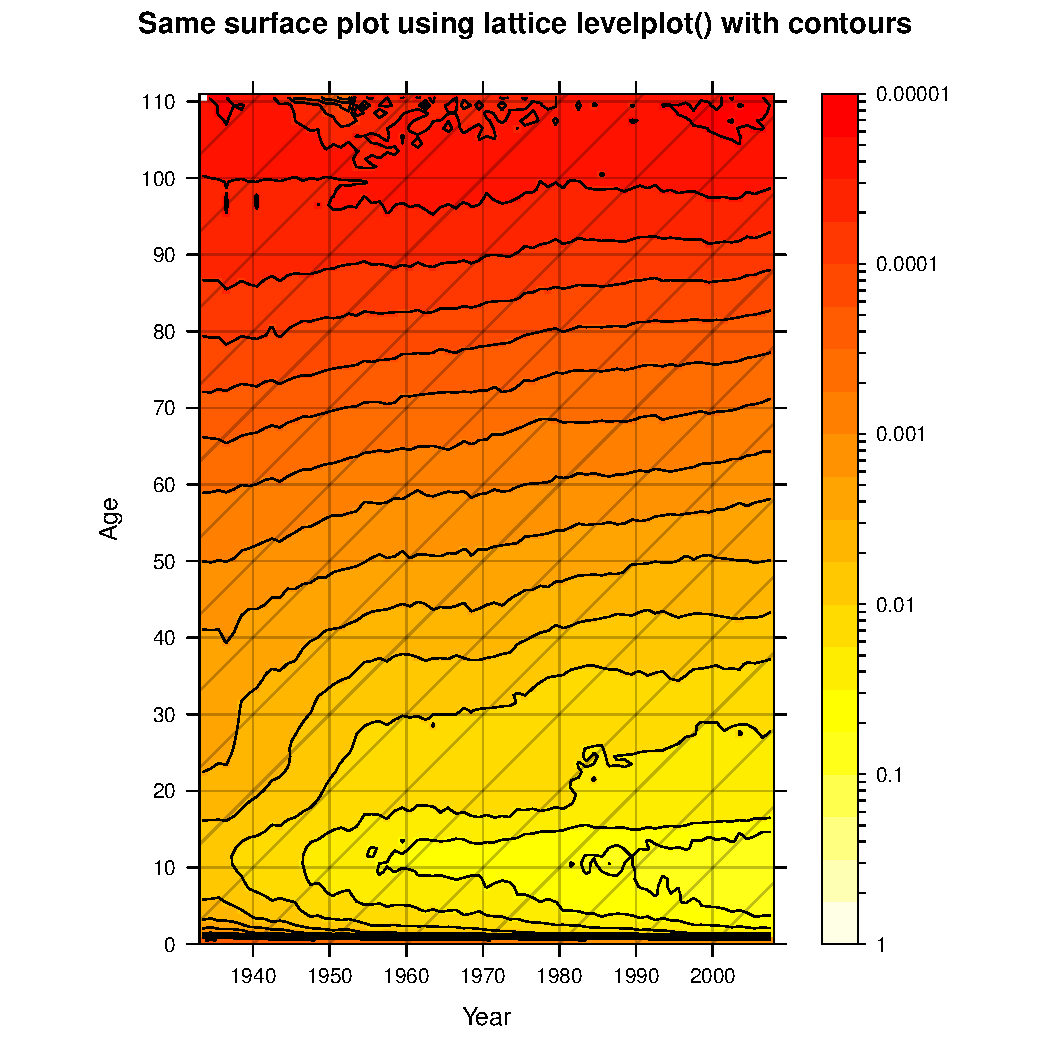
\includegraphics[width=4.5in,height=4.5in]{figs/latticegoodcontour.pdf}
\caption{\texttt{levelplot()} function, tweaked to produce a Lexis surface, with $\texttt{contour=TRUE}$.}
\end{figure}


This concludes our brief foray into \texttt{lattice} territory. Notice this took considerably fewer lines of code to produce than did the nearly identical \texttt{image()} version. The only drawback is the extra time spent having to learn its idioms, as opposed to brute force intuitive base graphics.
